
\chapter{Matrix Factorization Methods}  

Note:  The reader may find it useful to review Section \ref{partmat}
before continuing.

This chapter covers one of the more popular RS methods, matrix
factorization.  The overall theme will be \textit{low-rank
approximation}:  given a matrix $M_1$,  find a matrix $M_2$ for which 

\begin{equation}
rk(M_2) << rk(M_1)
\end{equation}

and 

\begin{equation}
M_2 \approx M_1
\end{equation}

This is important for \textit{dimension reduction}.  In RS, our
ratings matrix may have hundreds of millions of rows and millions of
columns, which presents both computational and overfitting problems.

To set the stage, we start with a more basic matrix operation, PCA.

\section{An Approach to Approximate Rank:  Principal Components
Analysis}

Suppose the matrix in (\ref{rankex1}) had been

\begin{equation}
\label{rankex2}  
M =
\left (
\begin{array}{rrrr}
1 & 5 & 1 & -2\\
8.02 & 2.99 & 2 & 8.2\\
9 & 8 & 3 & 6 
\end{array}
\right )
\end{equation}

Intuitively, we still might say that the rank of $M$ is
``approximately'' 2.  So row 3 still seems redundant, Let's
formalize that, leading to one of the most common techniques in
statistics/machine learning.  

The reason this is of interest is dimension reduction.  We would like to
reduce our feature set from $p$ variables to $s$, with $s << p$, with
the goal of avoiding overfitting.

\subsection{Exploiting Correlations}
\label{explorecorr}

Statistically, the issue is one of correlation.  In (\ref{rankex2}), the
third row is highly correlated with (the sum of) the first two rows.  To
explore the correlation idea further, recall our two graphs of bivariate
normal densities from Section \ref{mvnormal}:

\begin{minipage}[b]{0.65\linewidth}
    \mbox{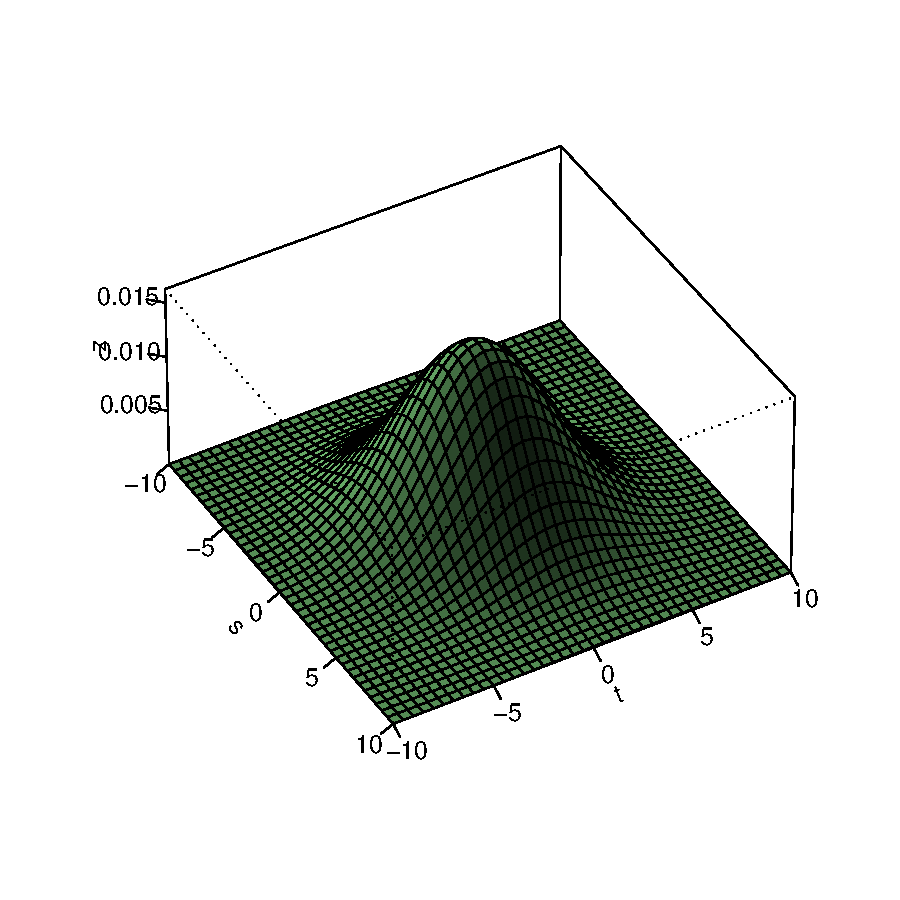
\includegraphics[width=3.25in]{Images/Rho2.pdf}} 
\end{minipage}
\hspace{0.0in}
\begin{minipage}[b]{0.65\linewidth}
    \mbox{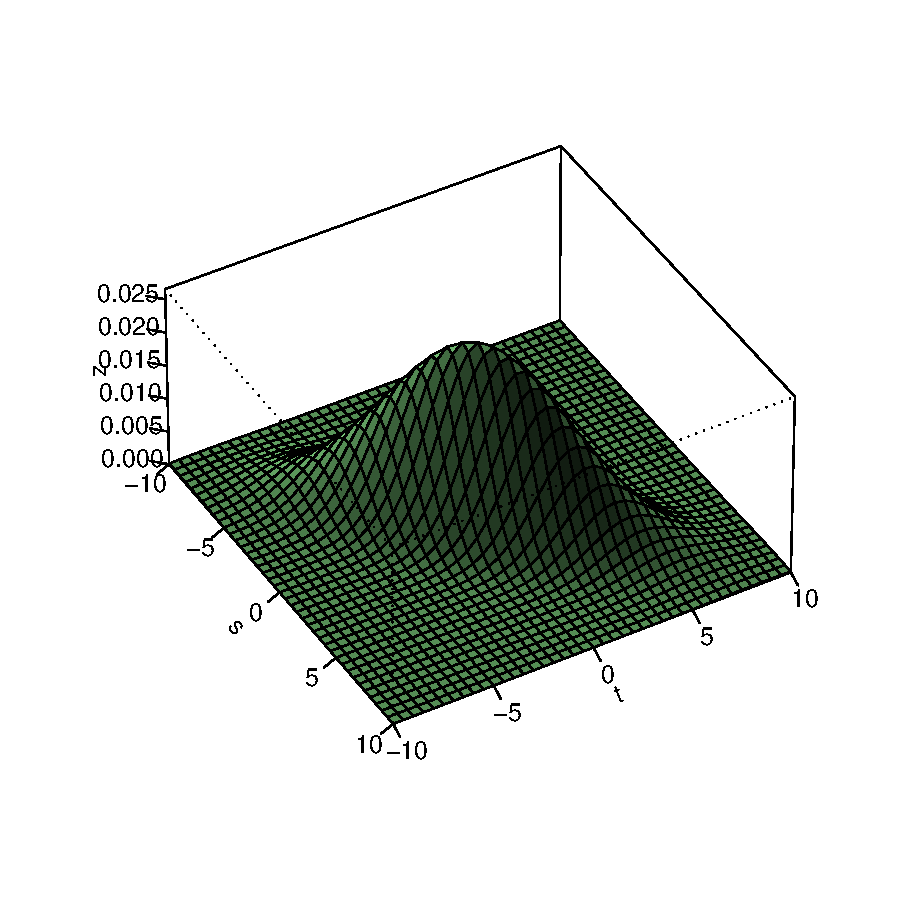
\includegraphics[width=3.25in]{Images/Rho8.pdf}} 
\end{minipage}

The two plots were for a low-correlation (0.2) distribution and a
high-correlation (0.8) one.  As we said at the time about the latter:

\begin{quote}

The probability that $X_2 \approx X_1$ is high.  So, to a large extent,
there is only one variable here, $X_1$ (or other choices, e.g.\ $X_2$),
not two.  

\end{quote}

In the case of correlation 0.2, the two variables are more separate.
The probability that $X_2 \approx -X_1$ is lower here.

Note one more time, though, the approximate nature of the approach we
are developing.  There really \textit{are} two variables even in that
correlation 0.8 example.  By using only one of them, \textbf{we are
relinquishing some information.  But with the need to avoid overfitting,
use of the approximation may be a net win for us.}

Well then, how can we determine a set of near-redundant variables, so
that we can consider omitting them from our analysis?  Let's look at
those graphs a little more closely.

Any \textit{level set} in the above graphs, i.e.\ a curve one
obtains by slicing the bells parallel to the $(t_1,t_2)$ plane, can be
shown to be an ellipse.  As noted, the major axis of the ellipse will be
the line $t_1 + t_2 = 0$.  The minor axis will be the line perpendicular
to that, $t_1 - t_2 = 0$.  That suggests forming new variables,

\begin{equation}
W_1 = X_1 + X_2 
\end{equation}

and 

\begin{equation}
W_2 = X_1 - X_2 
\end{equation}

In fact, taking

\begin{equation}
A = 
\left (
\begin{array}{rr}
1 & 1 \\
1 & -1 \\
\end{array}
\right )
\end{equation}

in (\ref{covax}) shows that $\rho(W_1,W_2) = 0$.

Here is the point so far:

\begin{itemize}

\item The high value of $\rho(X_1,X_2)$ suggests that for this dataset,
``one variable is enough.''  Thus we might consider using just $X_1$
rather than $X_1$ and $X_2$.

\item Or, we might consider using $W_1$ for our one
variable.  

\end{itemize} 

Now suppose we have $p$ variables, $X_1,
X_2,...,X_p$, not just two.  If our data is on people, these variables
may be height, weight, age, blood glucose level, and so on, i.e.\    
$X$ = (height, weight, age, blood glucose level,...)'.  

$X$ is different for each person, so it is a random vector.  Let $C$
denote the $p \times p$ covariance matrix of $X$.

Note:  In our data, we will have $n$ people, each of which has a
different value of the vector $X$.  Our data is then a matrix (or data
frame) of $p$ columns, with the value of $X$ for person $i$ in column
$i$.  If we call the R function \textbf{cov()} on that matrix, we get
$\widehat{C}$, the estimate of $C$.

We want to create a new 4-dimensional random vector $W =
(W_1,W_2,W_3,W_4)'$, with each $W_i$ being some linear combination of
$X_1, X_2, X_3 \textrm{ and } X_4$.

We can no longer visualize in higher dimensions, but one can show that
the level sets will be $p$-dimensional ellipsoids.  These now have $p$
axes rather than just two, and we can define our $W_i$ is such a way
that 

\begin{itemize}

\item [(a)] The $W_i$ are uncorrelated.

\item [(b)] They are ordered in terms of variance:

\begin{equation}
Var(W_1) \geq Var(W_2) \geq ... \geq Var(W_p)
\end{equation}

\end{itemize} 

Now we have a promising solution to our dimension reduction problem.  In
(b) above, we can choose to use just the first few of the $W_i$,
omitting the ones with small variance since they are essentially
constants, uninformative.  And again, since the $W_i$ will be
uncorrelated, we are eliminating a source of possible redundancy among
them; after all, we are doing dimension reduction, i.e.\ we wish to
reduce the number of variables, so we don't want any redundant ones.

PCA won't be a perfect solution --- there is no such thing --- as might
be the case if the relations between variables is nonmonotonic.  A
common example is age and income, with mean income given age tending to be a
quadratic (or higher degree) polynomial relation.  But PCA is a very
common ``go to'' method for dimension reduction, and may work well even
in (mildly) nonmonotonic settings.

Note too that although we've motivated things here with multivariate
normal distributions, we haven't assumed it.  We are merely talking
about finding a set of uncorrelated variables that are linear functions
of our original ones.

Now, how do we find these $W_i$?


\subsection{Eigenanalysis}

So, we are interested in finding new variables that are linear
combinations of our original ones.  Let's look at the first one.  
We want to choose $u$ to maximize 

\begin{equation}
Var(u'X) = u' C u
\end{equation}

where we have used (\ref{covax}) with $A = u'$.

Of course, this maximization problem doesn't make sense in the form
stated, since we can just make $u$ larger and larger to make $Var(u'X)$
large.  We need a constraint, say norm 1, $u'u = 1$.   

This calls for the method of \textit{Lagrange multipliers}.  We redefine
that problem as maximizing 

\begin{equation}
u'Cu - \omega (u'u - 1)
\end{equation}

where $\omega$ is an artificial variable that enforces the constraint.
Then

\begin{equation}
\frac{d}{du} [u'Cu - \omega (u'u - 1)] = 2 Cu + 2 \omega u 
\end{equation}

Setting this to 0, we have

\begin{equation}
0 = (C - \omega I) u
\end{equation}

In other words,

\begin{equation}
Cu = \omega u
\end{equation}

Aha!  The vector $u$ would have to be an eigenvector of $C$.  

Let's call that vector $u_1$.  Then what about the second linear
combination, $u_2$?  Again we would find $u$ to maximize

\begin{equation}
Var(u'X) = u' C u
\end{equation}

with the constraintt

\begin{equation}
u'u = 1
\end{equation}

but now with the additional constraint that we want $u_2$ to be
uncorrelated with $u_1$.  Using (\ref{covax}), that means

\begin{equation}
u'u_1 = 0
\end{equation}

Using two-variable Lagrange, we would find that $u_2$ is also an
eigenvector of $C$.

Say we have a sample of $n$ observations on $p$ variables, say $p$
measurements on each of $n$ people.  The measurements are $X_1,...,X_p$.
For example, we might have $p=3$, with $X_1, ~ X_2, \textrm{ and } X_3$
being height, weight and age.  

% Let $X_{ik}$ be the value of $X_i$ on the $k^{th}$ person, $k = 1,...,n$.
% 
% The sample correlation between $X_i$ and $X_j$ is the sample
% analog of (\ref{rhodef}),
% 
% \begin{equation}
% \label{corrdef}
% \widehat{\rho} =
% \frac
% {\frac{1}{n} \sum_{k=1}^n (X_{ik}-\overline{X}_i)
% (X_{jk}-\overline{X}_j)}
% {s.d.(X_i) ~ s.d.(X_j)}
% \end{equation}
% 
% where the denominator is the product of the sample standard deviations
% of the two variables, and $\overline{X}_i)$ and $\overline{X}_j)$ are
% the sample means.  

Let $C$ denote the covariance matrix of $X_1,...,X_p$.  Note that
since $Cov(X_i,X_j) = Cov(X_j,X_i)$, 
the matrix $C$ is \emph{symmetric},

\begin{equation}
C' = C
\end{equation}

% Recall that for any square matrix $L$, if there is a scalar $\lambda$
% and a nonzero vector $x$ such that 
% 
% \begin{equation}
% Lx = \lambda x
% \end{equation}
% 
% then we say that $x$ is an \textit{eigenvector} of $L$, with
% \textit{eigenvalue} $\lambda$.  

Another way of looking at the above derivation:

It can be shown\footnote{Here and below, ``can be shown'' means that the
assertion is proved in any standard textbook on linear algebra.} that
any symmetric matrix has real (not complex) eigenvalues, and that the
corresponding eigenvectors $U_1,...,U_p$ are \textit{orthogonal},

\begin{equation}
U_i' U_j = 0, ~ i \neq j
\end{equation}

We always take the $U_i$ to have length 1:  Just divide the vector by
its length, so it now has length 1, and is still an eigenvector.  

Let $U$ denote the $p \times p$ matrix whose $i^{th}$ column is $U_i$.
Then from the orthogonality of the eigenvectors, we have

\begin{equation}
\label{uui}
U'U = I
\end{equation}

so

\begin{equation}
U^{-1} = U'
\end{equation}

where $I is$ the $p \times p$ identity matrix.  We also refer to $U$ as
\emph{orthogonal}, for this property.

It also can be shown that 

\begin{equation}
U C U' = D
\end{equation}

where $D$ is a diagonal matrix with the eigenvalues of $C$ on the
diagonal.

% Multiplying on the left by $U'$ and the on the right by $U$,
% and using (\ref{uui}), we have
% 
% \begin{equation}
% C = U'DU
% \end{equation}


$X = (X_1,...,X_p)'$ is a random vector, i.e. different for each person
or other entity in the population.  Now, form a new random vector from
$X$:

\begin{equation}
W = UX
\end{equation}

Let's find its covariance matrix, again using (\ref{covax}):

\begin{equation}
Cov(W) = U C U' = D
\end{equation}

Aha!  The components of this new random vector are uncorrelated!  Just
what we need.  And that gives us PCA:

\subsection{PCA}

\begin{itemize}

\item Find the (sample) covariance matrix of $X$ in our data.

\item Diagonalize as above, yielding $U$ and $D$.

\item Reorder $D$ so that the eigenvalues are in nonincreasing order.
Reorder the rows of $U$ accordingly.

\item We are doing dimension reduction, reducing from $p$.  
Decide the new dimension $s$.

\item Replace $U$ by its first $s$ rows.

\item We've created a new random vector $W = UX$, with the new $U$.
$W$ will have length $s$, thus achieving dimension reduction.

\end{itemize} 

So for example, denote the $k^{th}$ value of $X$ in our original
dataset, i.e.\ column $k$, by $X^{(k)}$.  The corresponding new vector
is $W^{(k)} = U X^{(k)}$.  When dealing with a new case
$X^{(\textrm{new)}}$ in the future, premultiply by $U$ to get the $W$
value.


\subsection{Choosing the Number of Principal Components}  

The number of components we use, $s$, is a hyperparameter.  So, how do
we choose $s$?  

First one must ask what the goal of PCA is in the given application.
It might be simply descriptive; if we can reduce some complex set of
variables down to a few while losing only a small amount of
information, those remaining variables may give us insight into the
underlying workings of the process being studied.

For this goal, the (rather) standard approach is ``proportion of total
variance''; $s$ is chosen so that 

\begin{equation} 
\sum_{j=1}^s \lambda_j
\end{equation}

is ``most'' of total variance (that total is the above expression
with $p$ instead of $s$), but even this is usually done informally.

In ML/RS settings, though, $s$ is typically chosen by 
cross validation.  Say we are predicting $Y$ from $X = (X_1,...,X_p)'$,
using a linear model.  We fit such a model, predicting $Y$
from $W_1$ alone; then we predict $Y$ from only $W_1$ and $W_2$,
use then $s = 3$, then 4 and so on.  In each case, we look at our
prediction accuracy in our holdout set.  In the end, we use the value of
$s$ that gives the best accuracy.  The \textbf{qePCA()} function does
this.


\subsection{Software and UCI Repository Example}

The most commonly used R function for PCA is \textbf{prcomp()}.  As with
many R functions, it has many optional arguments; we'll take the default
values here.

For our example, let's use the Turkish Teaching Evaluation data,
available from the UC Irvine Machine Learning Data Repository.  It
consists of 5820 student evaluations of university instructors.  Each
student evaluation consists of answers to 28 questions, each calling for
a rating of 1-5, plus some other variables we won't consider here.

\begin{lstlisting}
> turk <- read.csv('turkiye-student-evaluation.csv',header=T)
> head(turk)
  instr class nb.repeat attendance difficulty Q1 Q2 Q3 Q4
1     1     2         1          0          4  3  3  3  3
2     1     2         1          1          3  3  3  3  3
3     1     2         1          2          4  5  5  5  5
4     1     2         1          1          3  3  3  3  3
5     1     2         1          0          1  1  1  1  1
6     1     2         1          3          3  4  4  4  4
  Q5 Q6 Q7 Q8 Q9 Q10 Q11 Q12 Q13 Q14 Q15 Q16 Q17 Q18 Q19
1  3  3  3  3  3   3   3   3   3   3   3   3   3   3   3
2  3  3  3  3  3   3   3   3   3   3   3   3   3   3   3
3  5  5  5  5  5   5   5   5   5   5   5   5   5   5   5
4  3  3  3  3  3   3   3   3   3   3   3   3   3   3   3
5  1  1  1  1  1   1   1   1   1   1   1   1   1   1   1
6  4  4  4  4  4   4   4   4   4   4   4   4   4   4   4
  Q20 Q21 Q22 Q23 Q24 Q25 Q26 Q27 Q28
1   3   3   3   3   3   3   3   3   3
2   3   3   3   3   3   3   3   3   3
3   5   5   5   5   5   5   5   5   5
4   3   3   3   3   3   3   3   3   3
5   1   1   1   1   1   1   1   1   1
6   4   4   4   4   4   4   4   4   4
> tpca <- prcomp(turk[,-(1:5)]
\end{lstlisting}

Let's explore the output.  First, the standard deviations of the new
variables:

\begin{lstlisting}
> tpca$sdev
 [1] 6.1294752 1.4366581 0.8169210 0.7663429 0.6881709
 [6] 0.6528149 0.5776757 0.5460676 0.5270327 0.4827412
[11] 0.4776421 0.4714887 0.4449105 0.4364215 0.4327540
[16] 0.4236855 0.4182859 0.4053242 0.3937768 0.3895587
[21] 0.3707312 0.3674430 0.3618074 0.3527829 0.3379096
[26] 0.3312691 0.2979928 0.2888057
> tmp <- cumsum(tpca$sdev^2)
> tmp / tmp[28]
 [1] 0.8219815 0.8671382 0.8817389 0.8945877 0.9049489
 [6] 0.9142727 0.9215737 0.9280977 0.9341747 0.9392732
[11] 0.9442646 0.9491282 0.9534589 0.9576259 0.9617232
[16] 0.9656506 0.9694785 0.9730729 0.9764653 0.9797855
[21] 0.9827925 0.9857464 0.9886104 0.9913333 0.9938314
[26] 0.9962324 0.9981752 1.0000000
\end{lstlisting}

This is striking.  The first principal component (PC) already accounts
for 82\% of the total variance among all 28 questions.  The first five
PCs cover over 90\%.  This suggests that the designer of the evaluation
survey could have written a much more concise survey instrument with
almost the same utility.

Now keep in mind that each PC here is essentially a ``super-question''
capturing student opinion via a weighted sum of the original 28
questions.  Let's look at the first two PCs' weights:

\begin{lstlisting}
> tpca$rotation[,1]
        Q1         Q2         Q3         Q4         Q5 
-0.1787291 -0.1869604 -0.1821853 -0.1841701 -0.1902141 
        Q6         Q7         Q8         Q9        Q10 
-0.1870812 -0.1878324 -0.1867865 -0.1823915 -0.1923626 
       Q11        Q12        Q13        Q14        Q15 
-0.1866948 -0.1862382 -0.1922729 -0.1911814 -0.1902380 
       Q16        Q17        Q18        Q19        Q20 
-0.1962885 -0.1808833 -0.1935788 -0.1927359 -0.1931985 
       Q21        Q22        Q23        Q24        Q25 
-0.1911060 -0.1908591 -0.1948393 -0.1931334 -0.1888957 
       Q26        Q27        Q28 
-0.1908694 -0.1897555 -0.1886699 
\end{lstlisting}

\begin{lstlisting}

> tpca$rotation[,2]
         Q1          Q2          Q3          Q4          Q5 
 0.35645673  0.23223504  0.11551155  0.24533527  0.20717759 
         Q6          Q7          Q8          Q9         Q10 
 0.20075314  0.24290761  0.24901577  0.12919618  0.18911720 
        Q11         Q12         Q13         Q14         Q15 
 0.11051480  0.21203229 -0.10616030 -0.15629705 -0.15533847 
        Q16         Q17         Q18         Q19         Q20 
-0.04865706 -0.26259518 -0.12905840 -0.15363392 -0.19670071 
        Q21         Q22         Q23         Q24         Q25 
-0.22007368 -0.22347198 -0.10278122 -0.06210583 -0.20787213 
        Q26         Q27         Q28 
-0.12045026 -0.07204024 -0.21401477 
\end{lstlisting}

The first PC turned out to place approximately equal weights on all 28
questions.  The second PC, though, placed its heaviest weight on Q1,
with substantially varying weights on the other questions.

While we are here, let's check that the columns of $U$ are orthogonal.

\begin{lstlisting}
> t(tpca$rotation[,1]) %*% tpca$rotation[,2]
              [,1]
[1,] -2.012279e-16
\end{lstlisting}

Yes, 0 (with roundoff error).  As an exercise in matrix partitioning,
the reader should run

\begin{lstlisting}
t(tpca$rotation) %*% tpca$rotation
\end{lstlisting}

then check that it produces the identity matrix $I$, then ponder why
this should be the case.

% \subsection{More on the PC Coefficients}
% \label{coors}
% 
% There is more to consider.
% 
% Do the PC coefficients have any interpretation?  The answer is
% probably no for ordinary people, but for the \textit{domain experts},
% very possibly yes.  In the teaching evaluation example above, a
% specialist in survey design or teaching methods may well be able to
% interpret the dominance of Q1 in the second PC.  A method called
% \textit{factor analysis}, an extension of PCA, is popular in social
% science research.
% 
% For the rest of us, PCA is just a handy way to do dimension reduction.
% 
% But there is geometric terminology that will be helpful, as follows.
% Let's look at the \textbf{mlb} dataset from the \textbf{regtools}
% package.  This is data on Major League baseball players.
% 
% \begin{lstlisting}
%              Name Team       Position Height Weight   Age
% 1   Adam_Donachie  BAL        Catcher     74    180 22.99
% 2       Paul_Bako  BAL        Catcher     74    215 34.69
% 3 Ramon_Hernandez  BAL        Catcher     72    210 30.78
% 4    Kevin_Millar  BAL  First_Baseman     72    210 35.43
% 5     Chris_Gomez  BAL  First_Baseman     73    188 35.71
% 6   Brian_Roberts  BAL Second_Baseman     69    176 29.39
%   PosCategory
% 1     Catcher
% 2     Catcher
% 3     Catcher
% 4   Infielder
% 5   Infielder
% 6   Infielder
% \end{lstlisting}
% 
% Let's apply PCA:
% 
% \begin{lstlisting}
% > hw <- as.matrix(mlb[,4:5]) 
% > pcout <- prcomp(hw) 
% > pcout$rotation 
%                PC1         PC2
% Height -0.05948695  0.99822908
% Weight -0.99822908 -0.05948695
% \end{lstlisting}
% 
% If we were to plot \textbf{hw}, we would put \textbf{hw[1,]} at the
% point (74,180) on our graph.  Recall from high school math that 74 and
% 180 are called the \textit{coordinates} of \textbf{hw2[1,]}, with
% respect to our ``H axis'' and ``W axis.''
% 
% But in doing PCA, we are creating new axes, PC1 and PC2, which are
% rotated versions of the H and W axes.  (Hence the naming of the $U$
% matrix as ``rotation'' in the \textbf{prcomp()} return value.)  Let's
% find the coordinates of \textbf{hw[1,]} with respect to the new axes:
% 
% \begin{lstlisting}
% > hw[1,] %*% pcout$rotation
%            PC1     PC2
% [1,] -184.0833 63.1613
% \end{lstlisting}
% 
% So (74,180) has become (-184.1,63.2) under the new coordinate
% system.  Let's see what the angle of rotation is. We can do that by
% seeing where a point on the H axis rotates to.
% 
% \begin{lstlisting}
% > pc10 <- c(1,0) %*% pcout$rotation
% > pc10
%              PC1       PC2
% [1,] -0.05948695 0.9982291
% > (atan(pc10[2] / pc10[1])) * 180/pi
% [1] -86.58964
% \end{lstlisting}
% 
% Almost 90 degrees clockwise.

\subsection{Scaling}

Some analysts prefer to \textit{scale} the data before applying PCA.
For each column, we would subtract the column mean and divide by the
column standard deviation.  The column would now have mean 0.0 and
variance 1.0.

The rationale for doing this is that if PCA is applied to the original
data, variables with large variance will dominate.  And then units would
play a role; e.g.\ a distance variable would have more impact if it were
measured in kilometers than miles.

Scaling does solve this problem, but its propriety is questionable.
Consider a setting with two features, $A$ and $B$, independent, with
variances 500 and 2, respectively, and with mean 100 for both.  Let $A'$
and $B'$ denote these features after centering and scaling.

As noted, PCA is all about removing features with small variance, as
they are essentially constant. If we work with $A$ and $B$, we would of
course use only $A$. But if we work with $A'$ and $B'$, we would use
both of them, as they both have variance 1.0.

So, dealing with the disparate-variance problem (e.g. miles vs.\
kilometers) shouldn't generally be solved by ordinary scaling, i.e.\ by
dividing by the standard deviation.  An alternative is to divide each
column by its mean.  This addresses the miles-vs.-kilometers problem,
and makes sense in that a variance is large or small in relation to its
mean.

\subsection{Role of PCA in RS}

If in an RS application we have a very large number of covariates, one
possible remedy is to use PCA for dimension reduction.  A second role is
to lead us into related operation, SVD, next.

\section{SVD}

The \textit{Singular Value Decomposition} (SVD) is a generalization 
of PCA.  It has many applications, but will be especially valuable for
us in RS, as it can factor our ratings matrix into the product of a user
matrix and an item matrix.

\subsection{The Decomposition}

Let $A$ be any matrix, not necesarily square.  In fact, it is nonsquare
in typical applications, RS being a case in point.  Let $n$ and $m$
denote the numbers of rows and columns of $A$.
% Let $k$ denote $rk(A)$.  
Then there exist matrices $U$, $D$ and $V$ such that

\begin{equation}
\label{audv}
A = U D V'
\end{equation}

where:

\begin{itemize}

\item The dimensions of $U$, $D$ and $V$ are $n \times n$, $n \times m$
and $m \times m$.

\item $U$ and $V$ are orthogonal matrices, so that $U U' = I$ and $V'V =
I$.

\item $D$ is a diagonal matrix in the sense that $D_{ij} = 0$ whenever
$i \neq j$.  The diagonal elements are the \textit{singular values}.
Let $d_{i}$ denote the $i^{th}$ diagonal element in $D$,
$i = 1,2,...,\min(n,m)$.  One can construct the matrices so that the
singular values are nonnegative.

\end{itemize} 

By permuting the rows and columns of $A$, e.g.\ in MovieLens, permuting
the order of the users, and that of the movies, we can arrange things so
that the singular values appear in descending order.  We'll assume that
here.

Let $u_i$ and $v_i$ denote the $i^{th}$ columns in $U$ and $V$, 
respectively.  By expanding the multiplication in (\ref{audv}), we have

\begin{equation}
\label{rank1s}
A = \sum_{i=1}^{\min(n,m)} d_i  u_i v_i'
\end{equation}

% The rows of $U$ for an orthonormal basis for the row space of
% $A$.  Recall:  The latter is the subspace of $\mathcal{R}^{m}$
% consisting of all linear combinations of the rows of $A$.  An
% orthonormal basis consists of linearly independent vectors of norm 1.
% 
% The rows of $V$ for an orthonormal basis for the column space of $A$.

\subsection{Low-Rank Approximation}

Equation (\ref{rank1s}) then suggests how to accomplish dimension
reduction.  Remember, the $d_i$ are decreasing.\footnote{Technically,
nonincreasing, but typically there are no cases of equality.}  The last
few may be really tiny, so we can delete those terms, just as we
deleted the principal components with small variances.

Say we retain the first $r$ terms, with $r < \min(n,m)$.  That is
equivalent to

\begin{itemize}

\item Retaining the $r \times r$ ``northwest corner'' of $D$.

\item Retaining the first $r$ columns of $U$.

\item Retaining the first $r$ columns of $V$.

\end{itemize} 

Result:

\begin{itemize}

\item The new $U$, $D$ and $V$ will now be of dimensions
$n \times r$, $r \times r$ and $m \times r$.

\item The new product $UDV'$ will still have dimensions $n \times m$,
the same as $A$.  But, whereas we had

\begin{equation}
A = UDV'
\end{equation}

before, we now have

\begin{equation}
A \approx UDV'
\end{equation}

\item The new $UDV'$ will have rank $r$, hence the term
\textit{low-rank approximation}.  In fact, it can be shown to be the
best rank-$r$ approximation to $A$, in the sense that the Frobenius norm
(Section \ref{vecnorms}) of the difference is minimized:

\begin{equation}
\label{bestlow}
UDV' = \arg \min_Q \| A - Q\|_{F}
\end{equation}

over all $n \times m$ matrices $Q$ having rank $r$.

\end{itemize} 

Note that ALS is not guaranteed to converge.  It is simply a heuristic,
\textit{ad hoc} method.  But it has been found to work well, and
is quite popular.

\subsection{Back to RS}

Since $D$ is a diagonal matrix with nonnegative diagonal entries, it has
a square root, which we will denote as $D^{0.5}$---to obtain the square
root matrix, take the square of each diagonal value.  Then

\begin{equation}
A \approx (UD^{0.5}) (D^{0.5} V')
\end{equation}

So to obtain our desired factorization $A \approx WH$, we simply set

\begin{equation}
W = UD^{0.5}, ~ H = D^{0.5}V' ~ 
\end{equation}

In our RS context, the ratings matrix $A$ has missing values.  How can
we find $U$, $D$ and $V$?  

If the proportion of missing values is low, as in our House Voting data,
we can apply SVD to the intact rows of $A$, then treat the remaining
rows as new cases to be predicted (Section \ref{predictwh} below).

Otherwise, the answer is that numeric methods exist to find the
approximate SVD, based on the non-NA elements of $A$.  They involve
optimization of certain complicated quantities, using a nonlinear
optimization technique.  One such technique is \textit{Stochastic
Gradient Descent} (SGD), an iterative workhorse method in machine
learning.  It essentially sets derivatives to 0 and solves, but with
various refinements.  Of course, $U$, $D$ and $V$ will then turn out to
be different from what they would be if $A$ were intact.

\section{General Issues with Matrix Factorization Methods}  

There are many refinements of the SVD approach described above, and
indeed many other ways to achieve approximate factorization.  We'll
discuss other methods, later in this chapter.  

In all methods, we have

\begin{equation}
A \approx WH
\end{equation}

where $W$ is of dimensions $n \times r$,
$H$ is of dimensions $r \times m$, and both matrices are of rank $r$.
There are several issues to discuss.

\subsection{Bias, Variance and Overfitting}

There are $nr$ numbers in $W$, and $rm$ in $H$.  Treating our data as a
sample from a conceptual population---e.g.\ all moviegoers and all
movies---estimating only $r(n+m)$ values is much better than estimating
the much larger $nm$ ones.

But this depends on $r$, which is our tuning parameter/hyperparameter
for this method.  We have a classical tradeoff:

As $r$ grows, the variance increases, due to estimating more parameters,
but the bias decrases.  As usual, typically $r$ is chosen by
cross-validation.

\subsection{Regularization}

To some analysts, ``If it's random, then shrink it.''  Matrix
factorization is no exception.  In the context here, that means
shrinking both $W$ and $H$, and we choose them to minimize

\begin{equation}
\|A - WH\|_F + \gamma_1 \|W\|_F^2 + \gamma_2 \|H\|_F^2
\end{equation}

\subsection{``Bias'' Removal}

In machine learning circles, the term \textit{bias} as a second,
unrelated meaning beyond the ``bias-variance tradeoff'' context.
This second meaning refers to the $\beta_0$ term in (\ref{betadef}).
Recall that if we have no covariates, i.e.\ $p = 0$ in that equation,
$\beta_0$ reduces to $EY$, the unconditional mean of $Y$.  

We will discuss covariates shortly, but for now the point is that it is
customary to \textit{center} the $A$ ratings matrix by subtracting
means.  Let $m$, $m_{i \cdot}$, and $m_{\cdot j}$ denote the overall
mean rating, the mean for user $i$ and the mean for item $j$,
respectively.  Then the recommended approach is to first make the
adjustment

\begin{equation}
\label{adjust}
A_{ij} \leftarrow A_{ij} - (m_{i \cdot} + m_{\cdot j} -m)
\end{equation}

Then the factorizaiton is performed, and finally the adjustment is
``undone'':

\begin{equation}
\label{unadjust}
A_{ij} \leftarrow A_{ij} + (m_{i \cdot} + m_{\cdot j} -m)
\end{equation}

What is going on here?  First, the expression

\begin{equation}
m_{i \cdot} + m_{\cdot j} -m
\end{equation}

is motivated by the equivalent

\begin{equation}
\label{anova}
m + (m_{i \cdot} - m) + (m_{\cdot j} -m)
\end{equation}

which models the ratings as 

\begin{quote}

overall mean + effect due to user i + effect due to item j

\end{quote}

(Readers who are familiar with the \textit{analysis of variance}
should recognize this.)  The idea is then to do our matrix factorization
on the \textit{residual}, i.e.\ what is ``left over'' after prediction
by the model (\ref{anova}).

\subsection{Dealing with Covariates}

Why stop with just removing ``biases''?  We can go a step further and
account for user or item covariates.

The easiest approach to handling covariates is again to subtract (and
later add back) certain values, in this case those arising from a linear
or other regression model.  One would first put the data in (user ID,
iterm ID, rating, covariates) format, then run \textbf{lm()} or
whatever.  Each element of $A$, or better, each rating in the input
data, is then adjusted by subtracting the predicted value for that
element.  One would then perform matrix factorization to fill in the
ratings matrix, then finally add the predicted values back to the
result.

Another way used by some analysts would be to append user covariates as
new columns in the $A$ matrix, or item covariates as new rows.

\subsection{Predicting New Cases} 
\label{predictwh}

One drawback of matrix factorization methods is that there generally is
no direct method to handle new users or new items not in the original
data.  One must compute the entire factorization all over again.  This
may not be too problematic, though, as most numerical methods are easy to
update, rather than fitting from scratch.

One solution is to use a k-Nearest Neighbors analysis on the completed
matrix aComp.  Say we have a new case with ratings for a set of items, A, R
and Q, and we want to predict this case's rating of item W.  Suppose R,
Q and W were in the original dataset, and thus have columns in aComp.
We look at the R, Q and W columns of that matrix, restricting attention
to rows in which there is a rating for W.  We now find the k rows
closest to the R and Q values of our new case, and average the
corresponding W rating.  That will be our predicted rating for the new
user.  Of course, if the new user only has rated item A, there is not
much we can do except predict from covariates.

find the k rows
closest to the new case, and 
average their ratings.

\section{Interpretation of W and H}

One of the big advantages of matrix factorization methods is
interpretability.

For any matrix $Q$, let $Q_{i \cdot }$, $Q_{\cdot j}$, and $Q_{ij}$
denote row $i$, column $j$, and element $(i,j),$ respectively.  Note the
key relation, using the material in Section \ref{partmat}:

\begin{equation}
\label{byrow}
(WH)_{i \cdot} = \sum_{m=1}^k W_{im} H_{m \cdot}
\end{equation}

In other words, in (\ref{byrow}), we see that:

\begin{itemize}

\item The entire vector of predicted ratings by user $i$ can be
expressed as a linear combination of the rows of $H$.

\item The rows of $H$ can thus be thought of as synthetic
``users'' who are representative of users in general.  $H_{rs}$ is the
rating that synthetic user $r$ gives item $s$.

\item Row $i$ of $W$ then tells us information about User in that
sense.  Indeed, we might use this information as a set of covariates in
predicting ratings.

\end{itemize} 

Of course, interchanging the roles of rows and columns above, we have
that the columns of $W$ serve as an approximate basis for the columns of
$A$.  In other words, the latter become synthetic, representative items,
e.g.\ representative movies in the MovieLens data.

% \subsection{Relation to Recommender Systems}
% 
% Many RS methods are text-based or even image-based.  Say there is a new
% movie, not user ratings yet at all.  One might compare the movie
% studio's synopsis of the film with those of flims for which we have
% ratings data, and try to predict how well each user would like this
% film.
% 
% A more ambiitious approach would be to do the same for images in the film's
% ad trailer.

% \section{The R Package NMF}
% 
% The R package {\bf NMF} is quite extensive, with many, many options.  In
% its simplest form, though, it is quite easy to use.  For a matrix {\bf
% a} and desired rank {\bf k}, we simply run
% 
% \begin{lstlisting}
% > nout <- nmf(a,k)
% \end{lstlisting}
% 
% Here the returned value {\bf nout} is an object of class {\bf "NMF"}
% defined in the package.  It uses R's S4 class structure, with
% \lstinline{@} as the delimiter denoting class membership, as opposed to
% \$ as in the S3 case.  
% 
% As is the case in many R packages, {\bf "NMF"} objects contain classes
% within classes.  The computed factors are in {\bf nout@fit@W} and {\bf
% nout@fit@H}.
% 
% Let's illustrate it in an image context, using the following:
% 
% 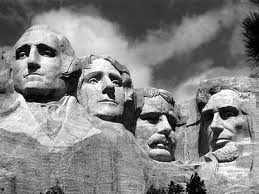
\includegraphics[width=3.6in]{Images/MtRush.png}
% 
% Here we have only one image, and we'll store it as a matrix $A$ (rows of
% the matrix corresponding to rows of $A$).  we'll use NMF to compress it,
% not do classification.  First obtain $A$:
% 
% \begin{lstlisting}
% > library(pixmap) 
% # read file
% > mtr <- read.pnm('MtRush.pgm') 
% > class(mtr)
% [1] "pixmapGrey"
% attr(,"package")
% [1] "pixmap"
% # mtr is an R S4 object of class "pixmapGrey"
% # extract the pixels matrix
% > a <- mtr@grey
% \end{lstlisting}
% 
% Now, perform NMF with rank 50, find the approximation to $A$, and
% display it:
% 
% \begin{lstlisting}
% > aout <- nmf(a,50)
% > w <- aout@fit@W
% > h <- aout@fit@H
% > approxa <- w %*% h
% # brightness values must be in [0,1]
% > approxa <- pmin(approxa,1) 
% > mtrnew <- mtr
% > mtrnew@grey <- approxa 
% > plot(mtrnew)  # dispatched to plot.pixmapGrey()
% \end{lstlisting}
% 
% Here is the result:
% 
% 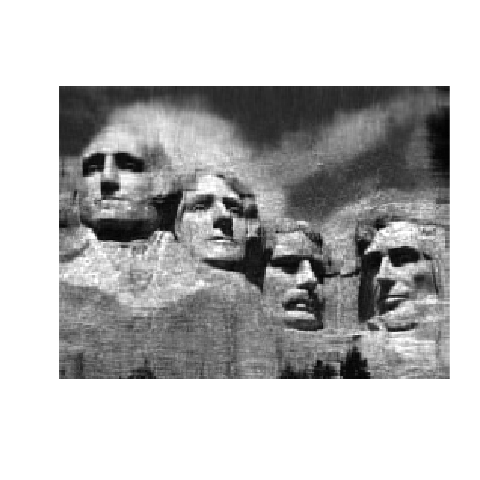
\includegraphics[width=3.6in]{Images/MtRush50.png}
% 
% This is somewhat blurry.  The original matrix has dimension $194 \times
% 259$, and thus presumably has rank 194.\footnote{One could check this by
% finding the number of nonzero eigenvalues of $A'A$, say by running
% \textbf{prcomp()}.} We've approximated the matrix by one of rank only
% 50.  We could use this for compression, and if we had millions of
% images and this amount of blurriness were acceptable, we could take this
% approach.
% 
% Actually, there are better ways to compress images, and this was just an
% illustration of the effect of the reduced rank.  Getting back to our
% classification context, the point is:
% 
% \begin{itemize}
% 
% \item When we use the term \textit{low-rank approximation}, it is indeed
% approximate, as can be seen by the blurriness.  
% 
% \item Applying NMF or PCA/SVD to a whole collection of images, e.g.\
% MNIST, further heightens this approximate nature of the process.
% 
% \item But we need to do something to avoid overfitting, i.e.\ some kind
% of dimension reduction, and finding a low-rank approximation does that.
% 
% \end{itemize} 
% 
% \section{The Bias vs.\ Variance Tradeoff}
% 
% The blurriness in that second picture is really an issue of bias, as
% follows.  Consider a given pixel, say in the 3rd row and 52nd column. 
% That pixel's intensity in the second picture will be a weighted
% average of various pixels in the first picture.  Some of the latter may
% be in locations within the picture that are somewhat far away from the
% 3rd row and 52nd column.  This biases the pixel in the second picture.
% 
% On the other hand, there definitely is a variance issue.  Let's review
% what this entails.
% 
% Recall from Chapter \ref{chap:overfit} that an intuitive way to view the
% variance issue in overfitting is that our data are being ``shared'' by
% the various things we're estimating, so that in a rough sense, each of
% these things has less data to itself.  Less data means more
% sample-to-sample variability, i.e.\ higher variance.  In linear
% regression with $p$ features, we are estimating $p+1$ parameters
% (including $\beta_0$); the larger $p$ is, the larger the variance of the
% estimated $\beta_i$.  Thus in turn we get larger variance to our
% predicted values.  For predicting a new case, different samples will
% give us different predictions, and larger $p$ will give us higher
% variance in our predicted value for that case.
% 
% Let $n$ and $m$ denote the number of rows and columns in $A$.  Then $W$
% and $H$ will be of dimensions $n \times k$ and $k \times m$.  Well,
% then, how many parameters are we estimating?  It's
% 
% \begin{equation}
% nk + km = k(n+m)
% \end{equation}
% 
% So, the larger we make $k$, the larger the variance.
% 
% In other words, in predicting a specific $A_{ij}$, our predicted value
% $\widehat{A}_{ij}$ will experience this tradeoff:
% 
% \begin{itemize}
% 
% \item Larger $k$ means lesser bias in our estimate of $\widehat{A}_{ij}$.
% 
% \item Larger $k$ means greater variance in $\widehat{A}_{ij}$.
% 
% \end{itemize} 
% 
% \section{Computation}
% \label{nmfcomp}
% 
% How are the NMF solutions found?  What is {\bf nmf()} doing internally?
% 
% Needless to say, the methods are all iterative, with one approach being
% that of the Alternating Least Squares algorithm AltLS).  It's quite
% intuitive, builds on our previous material and provides insight into NMF
% itself.\footnote{By the way, Alt.\ Least Squares is not the default for
% {\bf nmf()}.  To select it, set {\bf method = 'snmf/r'}.}
% 
% And most importantly ---  AltLS is easily adapted to the recommender
% systems setting.  Remember, recommender systems differ fundamentally
% from, say, the image and text classification applications cited earlier,
% due to the fact that some, typically the vast majority, of elements of
% the $A$ matrix are unknown.  
% 
% So let's take a look, still assuming for now that $A$ \textit{is}
% competely known.


\section{Alternating Least Squares (ALS)}

Again, a general approach to finding $W$ and $H$ is to minimize the
Frobenius norm of the approximation error:

\begin{equation}
\label{generalwh}
W,H = \arg \min_{w,h} \|A - wh\|_F
\end{equation}

Of course, minimizing that quantity is equivalent to minimizing its
square, setting up a least-squares approach that we'll describe here.
So, we wish to minimize

\begin{equation}
W,H = \arg \min_{w,h} \|A - wh\|_F^2
\end{equation}

As noted, we could use SGD for this.  But the old saying, ``Easier said
than done'' applies.  SGD works really well for minimization of
\textit{convex} functions.  Roughly, convexity means that a function
is concave-up in one dimension (i.e. the function has one argument),
``bowl-shaped'' in two dimensions (two arguments), and the
un-visualizable equivalent in multiple dimensions.  Unfortunately, 
the function

\begin{equation}
\label{fwh}
f(w,h) = \|A - wh\|_F^2
\end{equation}

which has $nr + rm$ arguments, is not convex.  And it generally will have
multiple local minima, causing possible convergence problems.

\subsection{A Non-SGD Approach, ALS}

For fixed $h$, the function $f(w,h)$ \textit{is} convex.  In fact, we
will see below that it's our old friend from the linear model, which not
only has a unique minimum but in fact has a closed-form solution for the
minimum!  The same is true if we fix $w$ and allow $h$ to vary.

The \textit{alternating least squares} approach to minimizing (\ref{fwh})
exploits the fact that $f(w,h)$ is separately convex in $w$ and $h$,
holding one of them fixed.  The algorithm is then

\begin{itemize}

\item [(1)] Set an initial guess $w_0$ for the solution.  (We won't need
an initial guess for $h$.)

\item [(2)] Minimize $f(w_0,h)$ with respect to $h$, yielding our next
guess, $h_1$.

\item [(3)] Minimize $f(w,h_1)$ with respect to $w$, yielding our next
guess, $w_1$.

\item [(4)] Minimize $f(w_1,h)$ with respect to $h$, yielding our next
guess, $h_2$.

\item [(5)] Repeat until convergence.

\end{itemize} 

Here is more detail:  In step (2) above, first write

\begin{equation}
\label{breakdownbyj}
f(w_0,h) = \sum_{j=1}^n
\|A_{\cdot j} - w_0 ~ h_{\cdot j}
\|_F^2
\end{equation}

where $h_{0 \cdot j}$ means column $j$ of $h_0$.  If we can find $h$ to
minimize the $j$ term in (\ref{breakdownbyj}) for each $j$, then we will
have minimized (\ref{breakdownbyj}) with respect to $h$, achieving our goal.

But luckily this is exactly the structure we had in minimizing
(\ref{quad}):

\begin{itemize}

\item The matrix $A$ there is our $w_0$ here, known.

\item The vector $D$ there is our $A_{\cdot j}$ here, known.

\item The vector $b$ there is our $h_{\cdot j}$ here, unknown and to be
solved for.

\end{itemize} 

So we have

\begin{equation}
(h_1)_{\cdot j} = (w_0'w_0)^{-1} w_0' A_{\cdot j}
\end{equation}

And again, via matrix partitioning,

\begin{equation}
\label{hfromw}
(h_1) = (w_0'w_0)^{-1} w_0' A
\end{equation}

for each $j$.  In later steps, $w_0$ is replaced by $w_i$.

% In R code,
% 
% \begin{lstlisting}
% > h[,j] <- lm(a[,j] ~ w0 - 1)$coef
% \end{lstlisting}

% The -1 specifies that we do not want a constant term in
% the model, i.e.\ no 1s column..

On the other hand, what about step (3)?.  We could take 
transposes,

\begin{equation}
A' \approx h' w'
\end{equation}

and then just interchange the roles of $w$ and $h$ above.  
Then (\ref{hfromw}) becomes something like

\begin{equation}
(w_1)_{i.} = (hh')^{-1} h A_{i.}
\end{equation}

One problem arises, though, in that the matrices may become of  
less than full rank (or close enough to it that R will declare them
singular).  What can be done?

\begin{itemize}

\item Again, some analysts feel, ``If it's random, shrink it.''  In this
context, it means that in ``predicting'' $A$ from $w$, we use 
using ridge regression instead of the ordinary linear model.  It can be
shown that this means adding $\lambda$ to the diagonal of $w'w$ before
taking the inverse.  So, we get shrinkage and invertibility, and
everyone is happy.

\item One can use what is called a \textit{generalized inverse}, or
\textit{pseudoinverste}.  This can be used not only to ``invert''
noninvertible matrices, but also even to ``invert'' non-square ones  And
in (\ref{hfromw}), it turns out (details not shown) that the $w$ factor
``cancel,'' giving us

\begin{equation}
(h_{i+1})_{\cdot j} = w_i^{+} A_{\cdot j}
\end{equation}

where for any matrix $Q$, the notation $Q^{+}$ means the generalized
inverse of $q$.

The R function \textbf{MASS::ginv()} does generalized inverse.  The
body of the iterative loop then, will look something like this (for the
matrix \lstinline{m} to be factored):

\begin{lstlisting}
      gw <- ginv(w)
      for (j in 1:ncol(m)) {
         h[,j] <- gw %*% m[,j]
      }
      gh <- ginv(t(h))
      for (i in 1:nrow(m)) {
         w[i,] <- t(gh %*% m[i,])
      }
\end{lstlisting}

\end{itemize} 

\subsection{Back to Recommender Systems:  Dealing with the Missing Values}

In our recommender systems setting, of course, much of $A$ is missing.
But we can easily adapt to that.  Roughly speaking, in
(\ref{breakdownbyj}), do these replacements:

\begin{itemize}

\item replace $A_{.j}$ by the known portion of $A_{.j}$

\item replace $w_0$ by the corresponding rows of $w_0$

\end{itemize} 

Note that $w_0$ will still have the same number of columns as before,
and thus there is no problem with conformability in multiplying
$h_{.j}$.

Then proceed as before.  

% Here is a little example.  Say $A$ ix $5 \times 5$ and we want rank 3.
% Then $W$ and $H$ are of sizes $5 \times 3$ and $3 \times5$.  
% 
% Note too that $(WH)_{.j}$, thus column $j$ of our approximation to $A$,
% is a linear combination of the columns of $W$, with coefficients being
% $H_{.j}$.
% 
% 
% Suppose
% 
% \begin{equation}
% A_{.4} = 
% \left (
% \begin{array}{r}
% NA \\
% 3 \\
% NA \\
% 8 \\
% 2
% \end{array}
% \right )
% \end{equation}
% 
% Then in (\ref{errajwhj}) we replace $A_{.5}$ by
% 
% \begin{equation}
% \label{smalla}
% \left (
% \begin{array}{r}
% 3 \\
% 8 \\
% 2 
% \end{array}
% \right )
% \end{equation}
% 
% Also, replace $W$ by
% 
% \begin{equation}
% \label{smallw}
% \left (
% \begin{array}{rrr}
% w_{21} & w_{22} & w_{23} \\
% w_{41} & w_{42} & w_{43} \\
% w_{51} & w_{52} & w_{53} \\
% \end{array}
% \right )
% \end{equation}
% 
% Remember, at this stage, $W$ is assumed known.  So, we just use
% \textbf{lm()}, ``predicting'' (\ref{smalla}) from (\ref{smallw}) to find
% $h_{.4}$.


% \subsubsection{Multiplicative Update}
% 
% Alternating Least Squares is appealing in several senses.  At each
% iteration, it is minimizing a {\it convex} function, meaning in essence
% that there is a unique local and global minimum; it is easy to
% implement, since there are many least-squares routines publicly
% available, such as {\bf lm()} here; and above all, it has a nice
% interpretation, predicting columns of $A$.
% 
% Another popular algorithm is {\it multiplicative update}, due to Lee and
% Seung.  Here are the update formulas for $W$ given $H$ and {\it vice
% versa}:
% 
% \begin{equation}
% W \leftarrow W \circ 
% \frac
% {AH'}
% {WHH'}
% \end{equation}
% 
% \begin{equation}
% H \leftarrow H \circ 
% \frac
% {W'A}
% {W'WH}
% \end{equation}
% 
% where $Q \circ R$ and $\frac{Q}{R}$ represent \underline{elementwise}
% multiplication and division with conformable matrices $Q$ and $R$, and
% the juxtaposition $QR$ means ordinary matrix multiplication.

\subsection{Convergence and Uniqueness Issues}

There are no panaceas for applications considered here.  Every solution
has potential problems.  I like to call this the Pillow Theorem ---
pound down on one fluffy part and another part pops up.

One issue with finding $W$ and $H$ by minimizing (\ref{generalwh}) is
uniqueness --- there might not be a unique pair $(W,H)$ that minimizes
(\ref{generalwh}).  In fact, one can see this immediately:  Doubling $W$
while halving $H$ leaves the product $WH$ unchanged.  Of course, the
product is all that really counts, but in turn, this may result in
convergence problems. Software documentation (see below) recommends
running the computation multiple times; it will use a different seed for
the random initial values each time.

Actually, the Alternating Least Squares method used here is considered
by some to have better convergence properties, since the solution at
each iteration is unique.  This may come at the expense of slower
convergence.

\section{Nonnegative Matrix Factorization (NMF)}

In most RS applications, the ratings are nonnegative.  So, we might
require that $W$ and $H$ be nonnegative.  

\subsection{Computation}

In ALS, for instance, we might just truncate to 0 any elements in $w_i$
and $h_i$ that stray into negative territory.  

Another popular approach is {\it multiplicative update}, due to Lee and
Seung.  Here are the update formulas for $W$ given $H$ and {\it vice
versa}:

\begin{equation}
W \leftarrow W \circ 
\frac
{AH'}
{WHH'}
\end{equation}

\begin{equation}
H \leftarrow H \circ 
\frac
{W'A}
{W'WH}
\end{equation}

where $Q \circ R$ and $\frac{Q}{R}$ represent \underline{elementwise}
multiplication and division with conformable matrices $Q$ and $R$, and
the juxtaposition $QR$ means ordinary matrix multiplication.  


\subsection{Why Nonnegative?}

NMF makes sense since the ratings are nonnegative, and also there is
hope that the resulting $W$ and $H$ are more likely to be sparse.

A second motivation is as follows:  Matrix factorization methods have
also been applied to image and text classification.  Consider 
a facial image recognition case, say.  There is hope that 
the nonzero elements of $W_{\cdot 1}$, say, correspond to eyes, $W_{\cdot
2}$ correspond to noses, and so on with other parts of the face.  We are
then ``summing'' to form a complete face.  This may enable effective
{\it parts-based recognition}, with helpful interpretations.

In our recommender systems setting, this parts-based effect, NMF would
give us crisper distinction among the various synthetic users.  This may
reveal clusters of user behavior, which could be quite helpful to the
analyst.

\section{Software}

Given that matrix factorization plays a major role in RS and many other
applications, it's not surprising that many libraries have been
developed for it.

\subsection{The svd() Function}

This is a general (i.e.\ not RS-specific) function to perform SVD.  The
function is part of base-R, and does not handle missing values.
Here is an example:

\begin{lstlisting}
> m
     [,1] [,2] [,3] [,4]
[1,]   15   18    5   11
[2,]    1   16   26    4
[3,]    5   12   13    5
> z <- svd(m)
> z
$d
[1] 40.9655903 18.1306964  0.3134599

$u
          [,1]        [,2]       [,3]
[1,] 0.5361629  0.80414164 -0.2566818
[2,] 0.7045689 -0.59380206 -0.3885637
[3,] 0.4648785 -0.02748343  0.8849478

$v
          [,1]       [,2]       [,3]
[1,] 0.2702611  0.6249570  0.5932112
[2,] 0.6469473  0.2561355 -0.6952051
[3,] 0.6601400 -0.6494748  0.3772584
[4,] 0.2695057  0.3492934  0.1498884
> z$u %*% diag(z$d) %*% t(z$v) 
     [,1] [,2] [,3] [,4]
[1,]   15   18    5   11
[2,]    1   16   26    4
[3,]    5   12   13    5
\end{lstlisting}

% \section{Functions in rectools}
% 
% The \textbf{recoSystem} package by Chih-Jen Li \textit{et al} has a good
% implementation of NMF for recommender systems (i.e.\ it handles the
% missing values).  However, it uses R6 classes (and is complicated in
% other ways), which are unfamiliar to many R users, so the
% \textbf{rectools} package provides wrappers.  Basic call forms are:
% 
% \begin{lstlisting}
% trainReco(ratingsIn,rnk=10,nmf=FALSE)
% predict.RecoS3(recoObj,testSet)
% \end{lstlisting}
% 
% Here \textbf{ratingsIn} is the usual three-column (userID,itemID,rating)
% (plus covariates, if any) data frame; \textbf{rnk} is the desired rank;
% \textbf{nmf} is false for SVD, true for NMF; \textbf{recoObj} is the 
% return value from \textbf{trainReco()}; and \textbf{testSet} is the test
% set, in the same format as \textbf{ratingsIn}, minus the ratings column.
% 
% The return value from \textbf{trainReco()} is an R S3 object of class
% 'RecoS3', with components $P$ and $Q$, corresponding to $W$ and $H'$ in
% our notation.  In the case of covariates (see below), some R
% \textbf{attributes} are also included.

\subsection{The recosystem Package}

The \textbf{recosystem} package does matrix factorization specifically
for recommender systems, i.e.\ specifically for settings in which the
matrix $A$ has many missing values.  It's written by experts in
numerical matrix factorization, and features a number of useful options.

The \textbf{recosystem} authors recognized that RS systems tend to be
large, with many rows and columns in a ratings matrix.  Accordingly, the
package does the following:

\begin{itemize}

\item It takes its input in the usual (user ID, item ID, rating) format,
not the ratings matrix, which could be huge.

\item As an option, it will stores the resulting $W$ and $H$ matrices as
disk files, rather than writing them to memory.

\end{itemize} 

The package uses R's R6 class system.  This is transparent if one uses
the wrapper \textbf{rectools::trainReco()}, but let's take a close look,
calling the function directly.


Below is a \textbf{recosystem} session using the small MovieLens data,
in the \textbf{ml100} data frame we've analyzed before.

Let's suppose we've decided on rank $k = 20$. 

\begin{lstlisting}
> library(recosystem)

> r <- Reco()
> class(r)
[1] "RecoSys"
attr(,"package")
[1] "recosystem"
# all action will take place within this R6 class instance; typically the 
# output of a function will be stored back as a new component in r

# need to create an object of class 'DataSource', specifying which
# columns are user IDs, item IDs and ratings; here we will have the data
# in memory; see below
> ml.dm <- data_memory(ml100[,1],ml100[,2],ml100[,3],index1=TRUE)

# do the factorization, with rank 20; use NMF not SGD
> r$train(ml.dm,opts=list(dim=20,nmf=TRUE))
iter      tr_rmse          obj
   0       2.0381   5.0056e+05
   1       1.0296   1.7402e+05
   2       0.9529   1.6028e+05
   3       0.9449   1.5868e+05
   4       0.9418   1.5811e+05
   5       0.9397   1.5774e+05
   6       0.9382   1.5749e+05
   7       0.9371   1.5729e+05
   8       0.9362   1.5713e+05
   9       0.9355   1.5701e+05
  10       0.9348   1.5690e+05
  11       0.9343   1.5681e+05
  12       0.9338   1.5673e+05
  13       0.9334   1.5666e+05
  14       0.9330   1.5660e+05
  15       0.9327   1.5654e+05
  16       0.9324   1.5649e+05
  17       0.9321   1.5645e+05
  18       0.9318   1.5641e+05
  19       0.9316   1.5637e+05
# training went for 20 iterations; RMSE is the square root
# of MSPE
# for large data, write to disk; here we store in memory
> result <- r$output(out_memory(),out_memory())
> str(result)
List of 2
 $ P: num [1:943, 1:20] 0.676 0.677 0.574 0.836 0.574 ...
 $ Q: num [1:1682, 1:20] 0.712 0.614 0.568 0.645 0.612 ...
# P and Q are W and H'
> w <- result$P
> h <- t(result$Q)
# let's try a prediction, with a known rating; we can do the
# matrix multiply ourselves if we wish
> head(ml)
   V1  V2 V3        V4
1 196 242  3 881250949
2 186 302  3 891717742
3  22 377  1 878887116
...
> w[22,] %*% h[,377]
         [,1]
[1,] 2.196976
# there is a predict() method, not shown here
\end{lstlisting}

Various options are available, such as regularization parameters.

\section{The softImpute Package}

In the literature on missing values, we often sees the term
\textit{impute}, which is a fancy form of ``guess.''  Hence the name of
this package.

The package works directly on the ratings matrix $A$.  If that matrix is
too large for memory, there is an option to use the Spark system, which
has an R interface \textbf{sparkr}.  Spark is a highly complex system
which may be difficult to install.  We do not pursue that here.

The user has a choice of ALS or SVD, default value of ALS, though in
both cases the algorithms used are refinements of what we see here.

Again, let's use MovieLens as an example:

\begin{lstlisting}
> mlm <- rectools::buildMatrix(ml100[,-4],NAval=NA)
> library(softImpute)
> z <- softImpute(mlm,rank.max=10)  # rank 10
> mlmest <- z$u %*% diag(z$d) %*% t(z$v)
# try a known rating
> head(ml100)
   V1  V2 V3        V4
1 196 242  3 881250949
2 186 302  3 891717742
3  22 377  1 878887116
4 244  51  2 880606923
5 166 346  1 886397596
6 298 474  4 884182806
> mlm[22,377]
[1] 1
> mlmest[22,377]
[1] 1.156759
\end{lstlisting}

